% Options for packages loaded elsewhere
\PassOptionsToPackage{unicode}{hyperref}
\PassOptionsToPackage{hyphens}{url}
%
\documentclass[
  10.5pt,
]{article}
\usepackage{amsmath,amssymb}
\usepackage{lmodern}
\usepackage{iftex}
\ifPDFTeX
  \usepackage[T1]{fontenc}
  \usepackage[utf8]{inputenc}
  \usepackage{textcomp} % provide euro and other symbols
\else % if luatex or xetex
  \usepackage{unicode-math}
  \defaultfontfeatures{Scale=MatchLowercase}
  \defaultfontfeatures[\rmfamily]{Ligatures=TeX,Scale=1}
\fi
% Use upquote if available, for straight quotes in verbatim environments
\IfFileExists{upquote.sty}{\usepackage{upquote}}{}
\IfFileExists{microtype.sty}{% use microtype if available
  \usepackage[]{microtype}
  \UseMicrotypeSet[protrusion]{basicmath} % disable protrusion for tt fonts
}{}
\makeatletter
\@ifundefined{KOMAClassName}{% if non-KOMA class
  \IfFileExists{parskip.sty}{%
    \usepackage{parskip}
  }{% else
    \setlength{\parindent}{0pt}
    \setlength{\parskip}{6pt plus 2pt minus 1pt}}
}{% if KOMA class
  \KOMAoptions{parskip=half}}
\makeatother
\usepackage{xcolor}
\usepackage[margin=1in]{geometry}
\usepackage{graphicx}
\makeatletter
\def\maxwidth{\ifdim\Gin@nat@width>\linewidth\linewidth\else\Gin@nat@width\fi}
\def\maxheight{\ifdim\Gin@nat@height>\textheight\textheight\else\Gin@nat@height\fi}
\makeatother
% Scale images if necessary, so that they will not overflow the page
% margins by default, and it is still possible to overwrite the defaults
% using explicit options in \includegraphics[width, height, ...]{}
\setkeys{Gin}{width=\maxwidth,height=\maxheight,keepaspectratio}
% Set default figure placement to htbp
\makeatletter
\def\fps@figure{htbp}
\makeatother
\setlength{\emergencystretch}{3em} % prevent overfull lines
\providecommand{\tightlist}{%
  \setlength{\itemsep}{0pt}\setlength{\parskip}{0pt}}
\setcounter{secnumdepth}{-\maxdimen} % remove section numbering
\newlength{\cslhangindent}
\setlength{\cslhangindent}{1.5em}
\newlength{\csllabelwidth}
\setlength{\csllabelwidth}{3em}
\newlength{\cslentryspacingunit} % times entry-spacing
\setlength{\cslentryspacingunit}{\parskip}
\newenvironment{CSLReferences}[2] % #1 hanging-ident, #2 entry spacing
 {% don't indent paragraphs
  \setlength{\parindent}{0pt}
  % turn on hanging indent if param 1 is 1
  \ifodd #1
  \let\oldpar\par
  \def\par{\hangindent=\cslhangindent\oldpar}
  \fi
  % set entry spacing
  \setlength{\parskip}{#2\cslentryspacingunit}
 }%
 {}
\usepackage{calc}
\newcommand{\CSLBlock}[1]{#1\hfill\break}
\newcommand{\CSLLeftMargin}[1]{\parbox[t]{\csllabelwidth}{#1}}
\newcommand{\CSLRightInline}[1]{\parbox[t]{\linewidth - \csllabelwidth}{#1}\break}
\newcommand{\CSLIndent}[1]{\hspace{\cslhangindent}#1}
\setlength\parindent{22pt}
\ifLuaTeX
  \usepackage{selnolig}  % disable illegal ligatures
\fi
\IfFileExists{bookmark.sty}{\usepackage{bookmark}}{\usepackage{hyperref}}
\IfFileExists{xurl.sty}{\usepackage{xurl}}{} % add URL line breaks if available
\urlstyle{same} % disable monospaced font for URLs
\hypersetup{
  pdftitle={Specific leaf area and leaf nitrogen content of Cecropia and Eschweilera},
  pdfauthor={Julia Rossi Mora},
  hidelinks,
  pdfcreator={LaTeX via pandoc}}

\title{Specific leaf area and leaf nitrogen content of \emph{Cecropia}
and \emph{Eschweilera}}
\usepackage{etoolbox}
\makeatletter
\providecommand{\subtitle}[1]{% add subtitle to \maketitle
  \apptocmd{\@title}{\par {\large #1 \par}}{}{}
}
\makeatother
\subtitle{Serrapilheira/ICTP-SAIFR Training Program in Quantitative
Biology and Ecology 2022: Computational methods}
\author{Julia Rossi Mora}
\date{August 2022}

\begin{document}
\maketitle

\hypertarget{introduction}{%
\subsection{Introduction}\label{introduction}}

\emph{Cecropia} is a genus of the family Urticaceae that consists of
species of pioneer trees (Berg, Rosselli, \& Davidson, 2005). The genus
\emph{Eschweilera} belongs to the family Lecythidaceae.

Plant functional traits are attributes that potentially affect
establishment, survival and fitness of plant individuals (Reich et al.,
2003). Two examples are specific leaf area (SLA) and leaf nitrogen
content.

Specific leaf area (SLA, i.e., leaf area per leaf dry mass) is an
inverse index of leaf density or thickness (Reich \& Walters, 1994). A
correlation between specific leaf area (SLA) and mass of nitrogen
(N\textasciitilde mass) has been previously identified in 23 Amazonian
tree species, one of them being \emph{Cecropia ficifolia}. In all
species analysed, across increasing leaf age and light gradients, SLA
decreased and so did N\textasciitilde mass, but proportionally slower,
in a way that N\textasciitilde area increased (Reich \& Walters, 1994).

In the study of Raaimakers et al.~(1995), nine tropical rainforest tree
species were defined as pioneer or climax, based on regeneration
strategy: \emph{Cecropia obtusa} was classified as a pioneer species and
\emph{Eschweilera sagotiana} as a climax species. The results showed
that, for tropical rainforest trees, pioneer species have higher leaf
phosphorus and nitrogen content in comparison to climax species
(Raaimakers, Boot, Dijkstra, \& Pot, 1995).

I formulated two hypothesis in the present study. The first hypothesis
is that the specific leaf area of \emph{Cecropia} is greater than that
of \emph{Eschweilera}. The second hypothesis is that the leaf nitrogen
content per leaf dry mass of \emph{Cecropia} is higher than that of
\emph{Eschweilera}.

\hypertarget{methods}{%
\subsection{Methods}\label{methods}}

For the current study, I used the package BIEN (Maitner, 2022), the
Botanical Information and Ecology Network, in RStudio (R Core Team,
2022). Firstly, all occurence records available in BIEN of
\emph{Cecropia} and \emph{Eschweilera} were ploted in a map. I gathered
the data of specific leaf area (SLA, i.e., leaf area per leaf dry mass)
of \emph{Cecropia} and \emph{Eschweilera} and created a boxplot to
better visualize them. The same was done for leaf nitrogen content per
leaf dry mass of both genera. I performed two Welch Two Sample t-tests,
one for each trait of both genera, in order to test if both have equal
means.

\hypertarget{results-and-discussion}{%
\subsection{Results and Discussion}\label{results-and-discussion}}

According to the database of BIEN, \emph{Cecropia} and
\emph{Eschweilera} are distributed in the Neotropics, but observations
of \emph{Cecropia} are more widely distributed than \emph{Eschweilera}
(for instance, there are no observations of \emph{Eschweilera} in
Argentina, Paraguay and south of Brazil in the database of BIEN) (Figure
1).

\begin{figure}
\centering
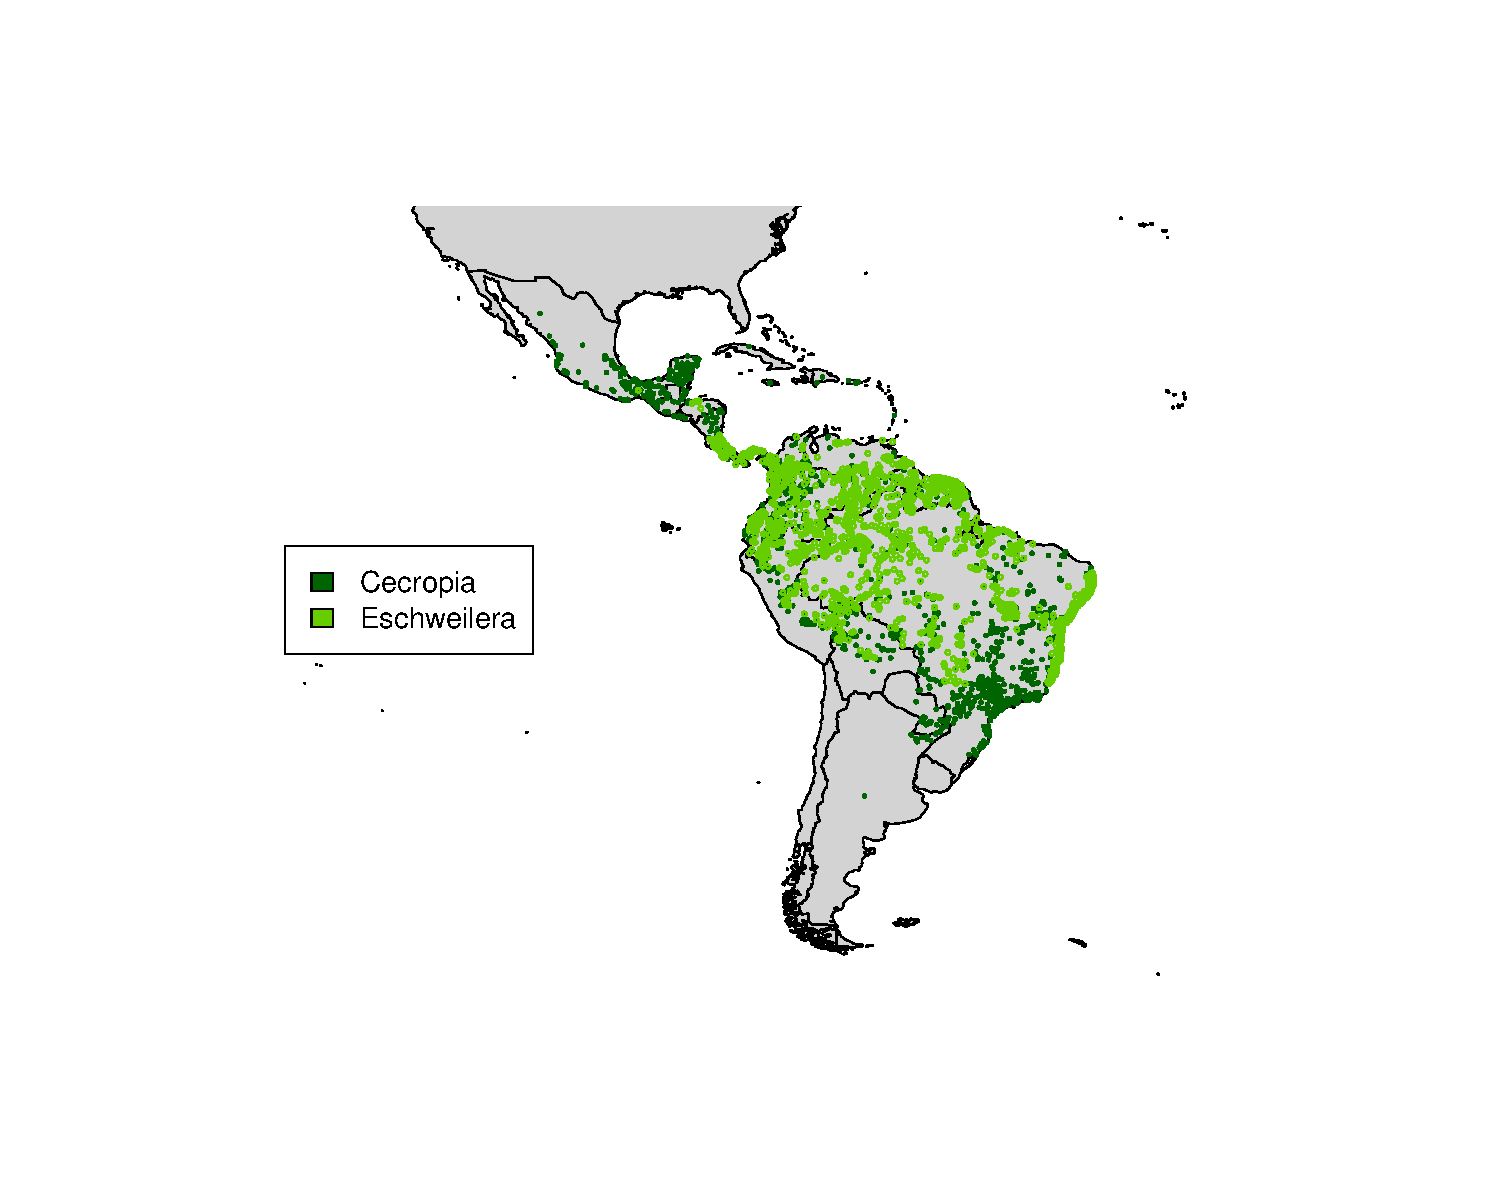
\includegraphics[width=0.65\textwidth,height=\textheight]{"../figs/map_occurence.pdf"}
\caption{Occurence map of \emph{Cecropia} and \emph{Eschweilera}.}
\end{figure}

For both genera, I loaded all available observations of the specific
leaf area (SLA) - i.e., leaf area per leaf dry mass. Figure 2 shows
these observations in boxplots.

\begin{figure}
\centering
\includegraphics[width=0.6\textwidth,height=\textheight]{"../figs/boxplot_sla.pdf"}
\caption{Specific leaf area (SLA) of \emph{Cecropia} and
\emph{Eschweilera}.}
\end{figure}

The Welch Two Sample t-test of the specific leaf area (SLA) of
\emph{Cecropia} and \emph{Eschweilera} resulted in: t = -5.2641, df =
78.642, p-value = 1.191e-06. The 95\% confidence interval is -8.889639
to -4.011222. Since the p-value is much smaller than 0.05, it is
possible to conclude that there is a statistically significant
difference between the means of SLA of the two genera.

The median of SLA of \emph{Cecropia} is 14.40105
m\textsuperscript{2}/kg, the mean is 15.51825 m\textsuperscript{2}/kg
and the standard deviation is 7.191866 m\textsuperscript{2}/kg. The
median of SLA of \emph{Eschweilera} is 22.8217 m\textsuperscript{2}/kg,
the mean is 21.96868 m\textsuperscript{2}/kg and the standard deviation
is 9.690317 m\textsuperscript{2}/kg. Thence, the median and the mean of
SLA of \emph{Cecropia} are smaller than those of \emph{Eschweilera}.

Therefore, the first hypothesis, that says that the specific leaf area
of \emph{Cecropia} is greater than that of \emph{Eschweilera}, was
refuted.

I also loaded all available observations of leaf nitrogen content per
leaf dry mass of \emph{Cecropia} and \emph{Eschweilera}. These
observations are shown in the boxplots of Figure 3.

\begin{figure}
\centering
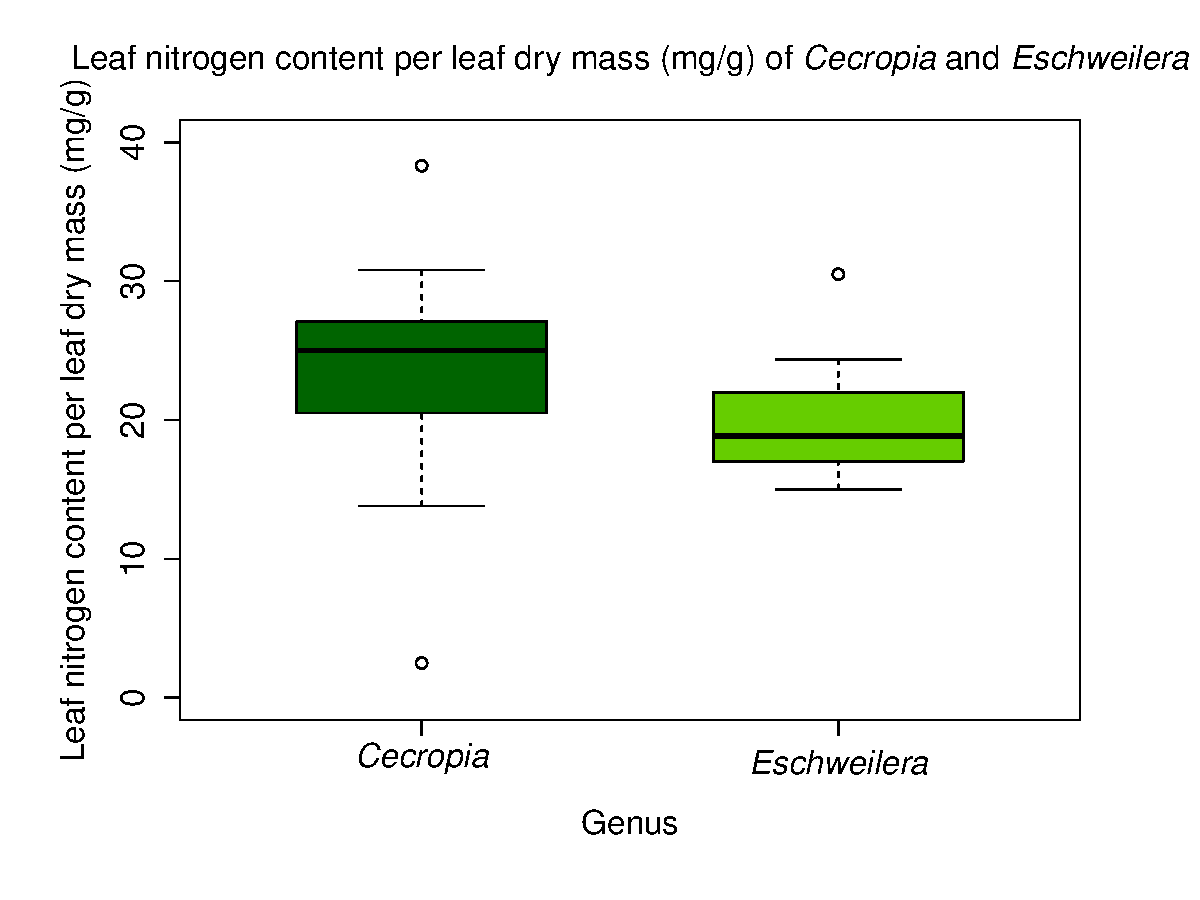
\includegraphics[width=0.6\textwidth,height=\textheight]{"../figs/boxplot_nitrogen.pdf"}
\caption{Leaf nitrogen content per leaf dry mass of \emph{Cecropia} and
\emph{Eschweilera}.}
\end{figure}

The Welch Two Sample t-test of leaf nitrogen content per leaf dry mass
of \emph{Cecropia} and \emph{Eschweilera} resulted in: t = 2.4205, df =
33.201, p-value = 0.02113. The 95\% confidence interval is 0.6461239 to
7.4481962. The p-value is smaller than 0.05, so there is also a
statistically significant difference between the means of leaf nitrogen
content per leaf dry mass of both genera.

The median of leaf nitrogen content per leaf dry mass of \emph{Cecropia}
is 25 mg/g, the mean is 23.72648 mg/g and the standard deviation is
7.09657 mg/g. The median of leaf nitrogen content per leaf dry mass of
\emph{Eschweilera} is 18.85 mg/g, the mean is 19.67932 mg/g and the
standard deviation is 3.65172 mg/g.

The results obtained corroborate the hypothesis that the leaf nitrogen
content per leaf dry mass of \emph{Cecropia} is higher than that of
\emph{Eschweilera}. It is possible that the particular morphology of
\emph{Cecropia} leaves had an impact in the results of this trait.

\hypertarget{references}{%
\subsection*{References}\label{references}}
\addcontentsline{toc}{subsection}{References}

\hypertarget{refs}{}
\begin{CSLReferences}{1}{0}
\leavevmode\vadjust pre{\hypertarget{ref-BergRosselliDavidson2005}{}}%
Berg, C. C., Rosselli, P. F., \& Davidson, D. W. (2005). Cecropia.
\emph{Flora Neotropica}, \emph{94}, 1--230. Retrieved from
\url{http://www.jstor.org/stable/4393938}

\leavevmode\vadjust pre{\hypertarget{ref-BIEN}{}}%
Maitner, B. (2022). \emph{BIEN: Tools for accessing the botanical
information and ecology network database}. Retrieved from
\url{https://CRAN.R-project.org/package=BIEN}

\leavevmode\vadjust pre{\hypertarget{ref-R2022}{}}%
R Core Team. (2022). \emph{R: A language and environment for statistical
computing}. Vienna, Austria: R Foundation for Statistical Computing.
Retrieved from \url{https://www.R-project.org/}

\leavevmode\vadjust pre{\hypertarget{ref-Raaimakersetal1995}{}}%
Raaimakers, D., Boot, R. G. A., Dijkstra, P., \& Pot, S. (1995).
Photosynthetic rates in relation to leaf phosphorus content in pioneer
versus climax tropical rainforest trees. \emph{Oecologia}, \emph{102},
120--125. doi:
\href{https://doi.org/10.1007/BF00333319}{10.1007/BF00333319}

\leavevmode\vadjust pre{\hypertarget{ref-ReichWalters1994}{}}%
Reich, P. B., \& Walters, M. B. (1994). Photosynthesis-nitrogen
relations in amazonian tree species. II. Variation in nitrogen vis-a-vis
specific leaf area influences mass- and area-based expressions.
\emph{Oecologia}, \emph{97}(1), 73--81. Retrieved from
\url{http://www.jstor.org/stable/4220589}

\leavevmode\vadjust pre{\hypertarget{ref-Reichetal2003}{}}%
Reich, P. B., Wright, I. J., Cavender‐Bares, J., Craine, J. M., Oleksyn,
J., Westoby, M., \& Walters, M. B. (2003). The evolution of plant
functional variation: Traits, spectra, and strategies.
\emph{International Journal of Plant Sciences}, \emph{164}(S3),
S143--S164. Retrieved from
\url{http://www.jstor.org/stable/10.1086/374368}

\end{CSLReferences}

\end{document}
